\documentclass{article}
 
\usepackage{amsmath}
\usepackage{amssymb}
\usepackage{listings}
\usepackage{graphicx}
\usepackage{subcaption}
\usepackage{mwe}
\usepackage{float}
\usepackage{epstopdf}
\usepackage[top=1.5in, bottom=1in, left=1in, right=1in]{geometry}


\title{Project 2 Advanced Land Finding Writeup}

\begin{document}
\maketitle
\section{Project Goals}

The goals / steps of this project are the following:\\\\
* Compute the camera calibration matrix and distortion coefficients given a set of chessboard images.\\
* Apply a distortion correction to raw images.\\
* Use color transforms, gradients, etc., to create a thresholded binary image.\\
* Apply a perspective transform to rectify binary image ("birds-eye view").\\
* Detect lane pixels and fit to find the lane boundary.\\
* Determine the curvature of the lane and vehicle position with respect to center.\\
* Warp the detected lane boundaries back onto the original image.\\
* Output visual display of the lane boundaries and numerical estimation of lane curvature and vehicle position.\\

\section{Write up}
In this section I will go over the pipeline code in project2.py
\subsection{Camera Calibration and Distortion Correction} 
The first step is to calibrate the camera using the provided figures using the defined function $cameraCalibration$ and $undistort$. \\
The first function defines object and find image points for camera calibration using $cv2.findChessboardCorners()$. The second function creates undistort images witg $cv2.calibrateCamera()$ and $cv2.undistort()$. An example of the figure before and after distortion correction is shown in Figure \ref{fig:1a} and Figure \ref{fig:1b} .

\begin{figure}
     \centering
     \begin{subfigure}[b]{0.4\textwidth}
         \centering
         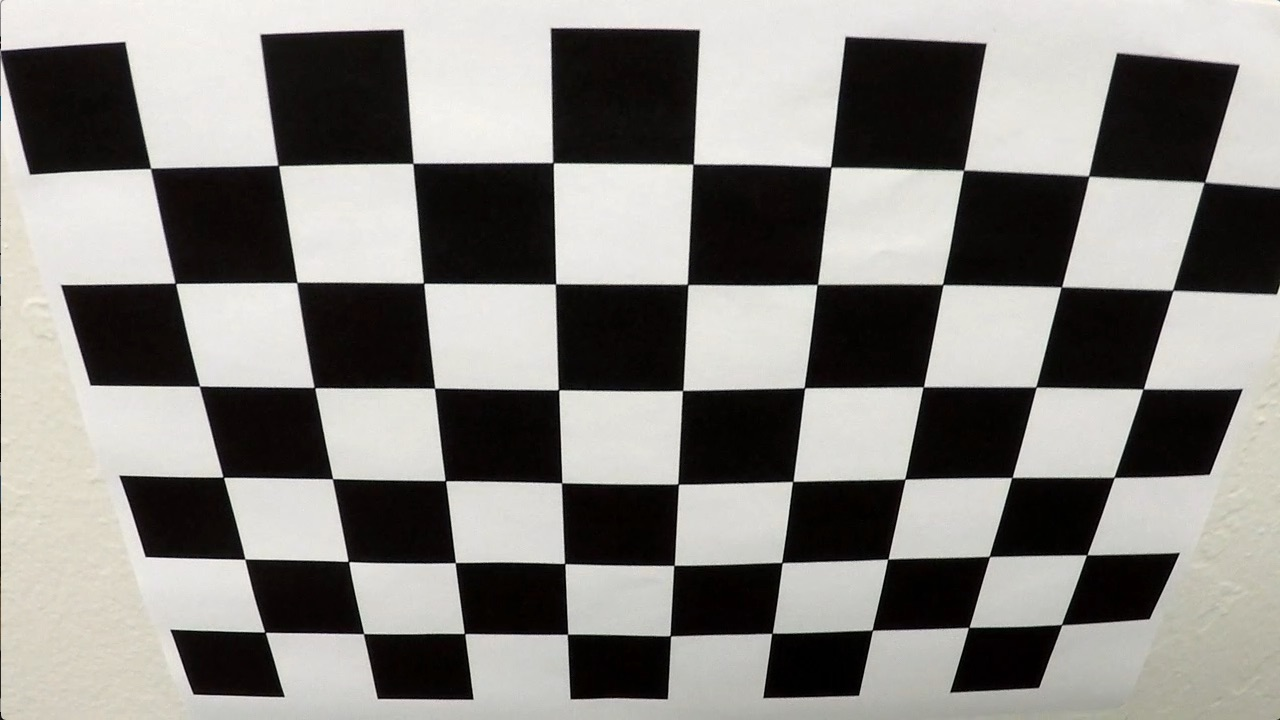
\includegraphics[width=\textwidth]{../camera_cal/calibration2.jpg}
         \caption{Before Distortion Correction}
         \label{fig:1a}
     \end{subfigure}
     \hfill
     \begin{subfigure}[b]{0.4\textwidth}
         \centering
         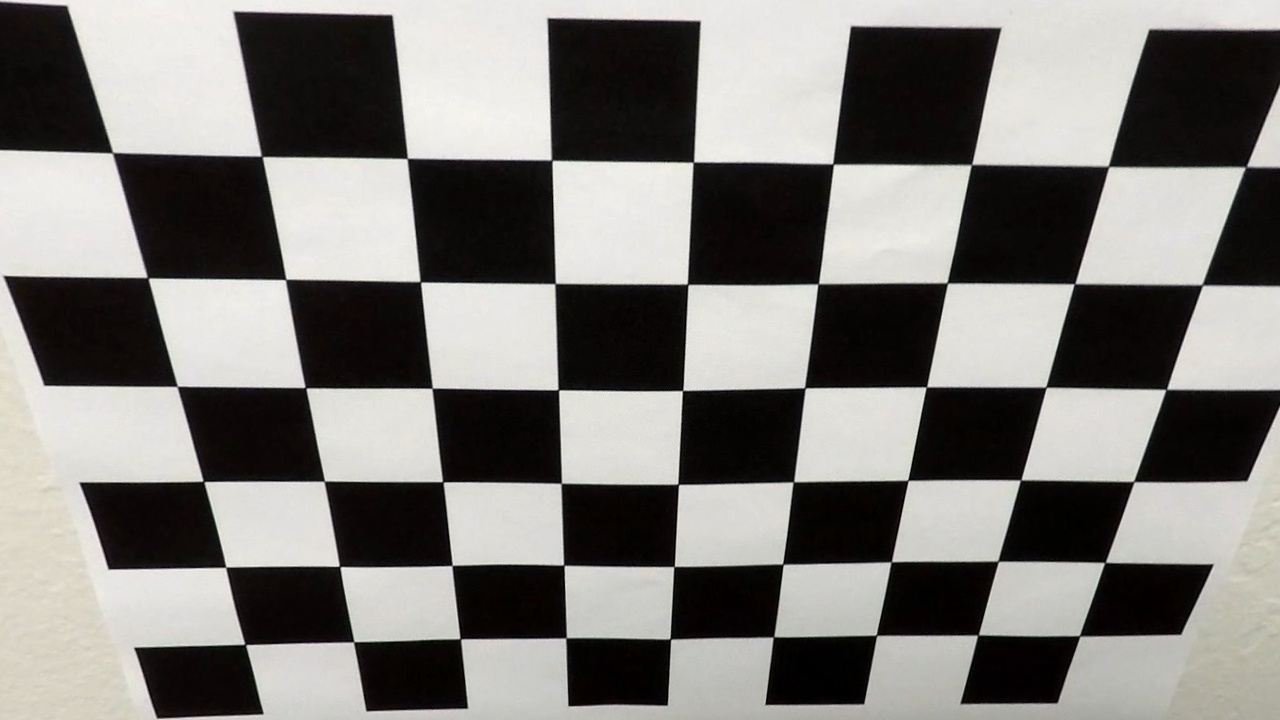
\includegraphics[width=\textwidth]{../output_images/undistort/alibration2.jpg}
         \caption{After Distortion Correction}
         \label{fig:1b}
     \end{subfigure}
\end{figure}
\subsection{Create Color Thresholded Image} 
The function $thresholdImage$ is used to create the binary threshold images

\end{document}
